\documentclass[letterpaper,12pt]{article}
\usepackage{geometry}
%package to include figures with .eps extension
\usepackage{graphics}
\geometry{paper=letterpaper,
                       body={6.50in, 9.00in},
                       lmargin=1.00in,
%                       rmargin=0.75in,
                       vmarginratio={1:1}
}
\begin{document}
\title{Intermediate Report -- Server Group}
\author{Ryan Wheeler, Shelby Lee, Patrick Green, Daniel Guilak}
\date{\today}
\maketitle
\newpage

\tableofcontents
\newpage

\section{Our Product}
The Server Team branch of the Vir-Pong project handles the communication between devices during a pong game, as well as the game logic. The server will function as the hub of communication for devices playing Vir-Pong, and will also maintain a database explicitly for the purpose of replaying games.

In the near future, devices will consist of modern browsers, Android platform phones, or Apple products running iOS with room for expansion on to other platforms as they become feasible. The server will determine the game logic -- such as ball movement and score -- as well as relay data such as paddle positions from each client. The system will also be able to facilitate live streaming of games to and from any client. The server will also provide an API for the WebUI team to access stored game replay files as well as other pertinent information such as user names and IDs. Also included will be detailed documentation on tools, references, and installation instructions.

\section{Functional Requirements}

\subsection{Use Cases}

\noindent \textbf{Scenario Title:}
\textbf{Version:} \\
\textbf{Actors:} \\
\textbf{Pre-conditions:}\\
\textbf{Post-conditions:}\\
\textbf{Scenario:}\\
\begin{enumerate}
\item
\end{enumerate}
\textbf{Alternatives:}\\
\textbf{1a.} 
\begin{enumerate}
\item
\end{enumerate}
\emph{Return}\\


\noindent \textbf{Scenario Title:} Any client connecting to system.\\
\textbf{Version:} 1.0\\
\textbf{Actors:} Client, network\\
\textbf{Pre-conditions:} Client has access to network, system is connected to network and accepting connections.\\
\textbf{Post-conditions:} Client is connected to system and ready to start a new game or join an existing one.\\
\textbf{Scenario:}
\begin{enumerate}
   \item Client requests connection with system.
   \item System accepts connection, assigns client a client ID.
   \item System sends client its ID and ready signal.
   \item System sends client information about current available games.
\end{enumerate}

\noindent \textbf{Scenario Title:} A client connecting to an open game.\\
\textbf{Version:} 1.1\\
\textbf{Actors:} Two clients, game state\\
\textbf{Pre-conditions:} Both clients have access to the network and are connected to the system and have been served the list of open games, one client is unpaired in an open game\\
\textbf{Post-conditions:}Clients are ready to play a game together\\
\textbf{Scenario:}
\begin{enumerate}
\item Client communicates to server which open game it wants to play.
\item System opens communication between client and client already in open game.
\item System initializes the game state.
\item The game is started
\item Paddle position is trasnmitted from client to the system
\item System transmits clients' paddle position, ball position, and score data back to client
\end{enumerate}
\textbf{Alternatives:}\\
\textbf{2a.} Client in open game rejects system request to start game 
\begin{enumerate}
\item System informs client that request to join was denied
\end{enumerate}
\emph{Return to 1}\\
\textbf{4a.} A client disconnects from the system
\begin{enumerate}
\item System freezes game state
\item System informs connected client of opponent disconnect
\item System prompts disconnected client for reconnect
\item System offers connected client to start new game
\item Connected client accepts new game
\item Game state is cleared
\item System informs disconnected client of game end
\end{enumerate}
\emph{Return to 1}\\

\noindent \textbf{Scenario Title:} Store player position in repository.\\
\textbf{Version:} 1.0\\
\textbf{Actors:} Client, system, repository, position tracker\\
\textbf{Pre-conditions:} System operational, client participating in game\\
\textbf{Post-conditions:} Game ends.\\
\textbf{Scenario:}
\begin{enumerate}
\item Client moves, position tracker sends data to system.
\item System communicates updated position to repository.
\item Repository logs position of client and adds time stamp.
\item Continues until system or client ends game.
\item System reports end of game to repository.
\item Repository logs end of game with time stamp.
\end{enumerate}


\noindent \textbf{Scenario Title:} Update player scores.\\
\textbf{Version:}1.1\\
\textbf{Actors:} Client1, Client2, Repository, Game Logic\\
\textbf{Pre-conditions:} System Operational, Client1 and Client2 logged in and participating in game \\
\textbf{Post-conditions:} Game continues\\
\textbf{Scenario:}
\begin{enumerate}
\item Client1 moves to hit the ball.
\item Game logic determines ball movement.
\item Client2 does not move 
\item Game logic determines no collision. 
\item Game logic pause game to informs system of client1 point.
\item System communicates point incrimination to game repository.
\item Game repository increments client1’s point.
\item Game repository communicates current score back to server.
\item Game repository sends current score to client interface.
\item Client interface displays current score
\end{enumerate}

\noindent \textbf{Scenario Title:} Accessing a replay from the repository.\\
\textbf{Version:} 1.0\\
\textbf{Actors:} Game Logic, Game repository, Interface\\
\textbf{Pre-conditions:} System operational.\\
\textbf{Post-conditions:} User interface shows a replay.\\
\textbf{Scenario:}
\begin{enumerate}
\item User chooses a game to watch.
\item Game repository selects requested game.
\item Position information from game repository sent to interface.
\item Position information is iterated over based on time stamp.
\item Game logic rebuilds ball positions based from recorded positions.
\item System sends data to user interface to be viewed.
\end{enumerate}

\noindent \textbf{Scenario Title:} Two clients with simple reactions are playing a game until a winner is determined. \\
\textbf{Version:}2.0\\
\textbf{Actors:} Two clients, game logic\\
\textbf{Pre-conditions:} System operationa, two clients connected to system, clients prepared to start game\\
\textbf{Post-conditions:} The game is complete\\
\textbf{Scenario:}
\begin{enumerate}
\item System pairs users
\item Game logic sets players and ball at default positions
\item System informs clients of game start
\item Game logic starts ball movement
\item System sends ball movement to both users
\item System recieves position data information from client
\item System informs game logic of movement
\item System sends position data to other client
\item Game logic determines no collision
\item User recieves a point\\ 
 \emph{Repeat 4 - 10 until score limit}
\item System informs client of score
\end{enumerate}
\textbf{Alternatives:}\\
\textbf{9a.} Game logic determines collision
\begin{enumerate}
\item Game logic recalibrates ball position based off of collision data
\item Game logic sends ball position to system
\end{enumerate}
\emph{Return to 5}\\


\noindent \textbf{Scenario Title:} Client plays against an artificially generated opponent.\\
\textbf{Version:}1.0\\
\textbf{Actors:} Client, game logic\\
\textbf{Pre-conditions:} Client has access to the network and is connected to the system\\
\textbf{Post-conditions:} Client is playing a game with artificial opponent\\
\textbf{Scenario:}
\begin{enumerate}
\item Client asks for offline game
\item System informs game logic of offline game
\item Client chooses opponent difficulty
\item Game logic generates artificial player's movement patterns
\item System prompts game start
\end{enumerate}


%Will probably have lots of \newpage commands here.
\subsection{System Sequence Diagram}
\section{Nonfunctional Requirements}
\begin{itemize}
\item The desired communication time between a phone and server should be process and stored with less than a 75 nanosecond lag-time.
\item The server should be able to handle at least 10 simultaneous conversations (games) without failure. 
\item If the server is unable to store game data, we will inform client so that the client may present the user with a message stating that the data will not be stored (high scores, replay information, etc.), but otherwise gameplay will remain unaffected. 
\item We will also plan on having two types of computer-programmed players. One will simply track ball movement, and the other with more randomization. 
\item Ideally we'd have players determine the size of the playing field, and that size would automatically create a ratio that fits to the client interface. 
\end{itemize}
These secondary features will bring out the performance and ability of our server and increase the game options Vir-Pong players are afforded. 
\section{Domain Analysis}
The domain of our problem consists largely of a client, game, and a lobby. We want the lobby, our conceptualization of a server, to connect clients to games.\\
\begin{center}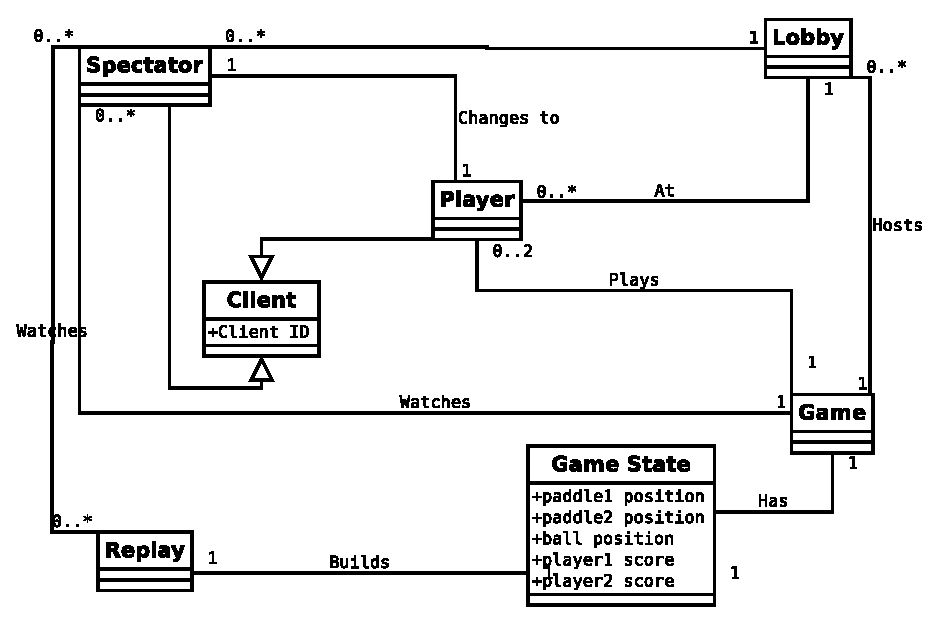
\includegraphics{DomAnaUML.eps} \end{center} 
A client is recognized mainly by the device used in connecting with the lobby. This device is assigned a clientID by the lobby in order to track user interactions with the system. At any one point in time, a client can be either a player or an observer. A client can easily switch between these definitions, but will always retain their clientID while connected. Such is why we have made player and spectators conceptual classes of the generic class client. A theoretically infinite amount of spectators can observe a game, but only two players can play one game. The lobby that connects players and observers to games can host a theoretically infinite amount of games at any one given moment, but all games are tagged back to one lobby. Each game is associated with a single game state. This game state holds the positions of the paddles and the ball. The game state only exists during an instance of the game and, quite essentially, holds the state of a game. Our definition of a game state is the position of paddles and the ball. This game state builds a replay. Any number of spectators can watch any number of these replays. 

\section{Implementation}
\subsection{Style Guide}
\subsubsection{Whitespace}
The basic indentation is two spaces. Tabs are not to be used at all.
Try to keep lines to 80 characters or less. When wrapping lines, try to indent to line up with a related item on the previous line. Examples: 
\begin{verbatim}
var result = prompt(aMessage,
                    aInitialValue,
                    aCaption);
\end{verbatim}
Lines should not contain trailing spaces, even after binary operators, commas or semicolons.
Separate binary operators with spaces.
Spaces go after commas and semicolons, but not before.
Spaces go after keywords. For example:
\begin{verbatim}
if (x > 0)
\end{verbatim}
One (or two) blank lines between block definitions. Also consider breaking up large code blocks with blank lines.

\subsubsection{Commenting}
Use multi-line comments to explain the purpose behind blocks of code.
Use in-line comments often to clarify actions.

\subsubsection{Symbols}
Function braces can either be on their own line or the open brace on the function declaration, i.e.

\begin{verbatim}
function toOpenWindow(aWindow)
  {
    aWindow.document.commandDispatcher.focusedWindow.focus();  
  }

function toOpenWindow(aWindow) {
    aWindow.document.commandDispatcher.focusedWindow.focus();  
}
\end{verbatim}
Spaces are not necessary inside brackets e.g. parameter lists, array subscripts.
Prefer double quotes, except in in-line event handlers or when quoting with double quotes ie (‘he said, “trouble” ’).
Have braces indented relative to their parent statement.
\subsubsection{Code Style}
Always put the else of an if-else statement on its own line.
Both i++ and ++i should not be used.
\subsubsection{Function and Varible Naming}
\begin{itemize}
\item Global variables should be prefixed with the letter g, e.g. var gFormatToolbar;
\item Arguments (parameter names) should be prefixed with the letter a.
\item Event handler functions should be prefixed with the word "on".
\item Function names, local variables and object members have no prefix.
\item Try to declare local variables as near to their use as possible; try to initialize every variable.
\end{itemize}

\subsubsection{JavaScript Features}
Make sure that your code doesn't generate any strict JavaScript warnings, such as:
\begin{itemize}
      	  \item{Duplicate variable declaration}
      	  \item{Mixing return; with return value;}
      	  \item{Trailing comma in JavaScript object declarations}
\end{itemize}    	
If you are unsure if an array value exists, compare the index to the array's length. If you are unsure if an object member exists, use "name" in aObject, or if you are expecting a particular type you may use typeof aObject.name == "function" (or whichever type you are expecting).
Use \{ member: value, ... \} to create a JavaScript object; a useful advantage over new Object() is the ability to create initial properties and use extended JavaScript syntax to define getters and setters.  If having defined a constructor you need to assign default properties it is preferred to assign an object literal to the prototype property. For example,

\begin{verbatim}
function SupportsString(data)
{
  this.data = data;
}
\end{verbatim}
Do not compare booleans to true or false. For example, write if (ioService.offline). Compare objects to null, numbers to 0 or strings to "" if there is chance for confusion.

\subsection{Install Documentation}
\subsubsection{Server}
Requirements:
\begin{itemize}
\item A relatively new machine (read: purchased/built in the last six years or so) running Linux or Mac OS X (These instructions were generated on a machine running Ubuntu 11.10 -- the configuration used for generation of instructions will henceforth be denoted in parentheses).
\item Basic Unix tools will already be installed, but other requirements that may not be present in a standard installation are:
Curl (using 7.21.6)
Git (using 1.7.5.4)
\item Connection to the Internet. 
\end{itemize}
Instructions:
Each line is a unix command, and so each of these commands must be typed into a shell of some sort, such as BASH or ZSH (using BASH). Alternatively, these commands can be easily generated into a BASH shell script quite easily of so desired.

To install node and the node package manager (npm):

\begin{verbatim}
echo 'export PATH=$HOME/local/bin:$PATH' >> ~/.bashrc
. ~/.bashrc
mkdir ~/local
mkdir ~/node-v0.4.9
cd ~/node-v0.4.9
curl http://nodejs.org/dist/node-v0.4.9.tar.gz | tar xz --strip-components=1
./configure --prefix=~/local
make install # ok, fine, this step probably takes more than 30 seconds...
curl http://npmjs.org/install.sh | sh
\end{verbatim}

To install the express web framework and socket.io:

\begin{verbatim}

npm install -g express socket.io #installs express server (expressjs.org) and socket.io
cd <your directory name>
express express-test && cd express-test
npm install -d #resolve dependencies
node app.js #runs test server with node
#point browser to localhost:3000 (default) -- should see welcome message
\end{verbatim}

To run the server:

First, clone the paddle-meister repository using git:

\begin{verbatim}
git clone git://github.com/VirPong/paddle-meister.git
\end{verbatim}

Then, navigate to the socket-test folder and execute

\begin{verbatim}
node server.js
\end{verbatim}

The server will run at whichever port specified in the PORT variable in server.js. To shutdown the server, press CTRL-C twice.

\subsubsection{MongoDB and Modules}
First go to mongodb.org and find the path to the most recent 64-bit Linux version. Then put this onto the server using shell commands:

\begin{verbatim}
wget [path copied from web]
\end{verbatim}
Then uncompress the file using tar with

\begin{verbatim}
tar zxvf [file name].tgz
\end{verbatim}

Then install MongoDB using the synaptic package manager (Debian-based Linux distributions only):
\begin{verbatim}
sudo apt-get install mongodb
\end{verbatim}

After looking over this open-source module, we determined that node-mongodb-native was perfectly suited for our project. This module facilitates a connection between mongodb and our server, which uses node. However, we ran into a compilation error when attempting to run example code, complaining of the native bson parser not being compiled.
In searching for a solution, we were pointed to another module for mongodb, called mongojs. Mongojs is actually a wrapper for mongodb-native that allows code to be written in a format almost identical to the mongodb shell API. This allows the code to be condense and clear.
We retrieved node-mongodb-native from github and mongojs was installed via npm with the shell command:

\begin{verbatim}
npm install mongojs
\end{verbatim}

\subsection{Algorithms, Data Structures, and Design Patterns}
\subsection{Design Pattern}
The node.js server framework is event-driven, so naturally design has been focused around creating and dealing with events.
For example, there are connect, disconnect, updatePaddle, startGame, and other such events that are implemented both server- and client-side.

\subsection{Data Storage}
The data we’re storing is specific to games and the players of each. This data is limited to usernames, player positions, gameIDs, and scores. This information will be stored in the noSQL database, mongodb. We choose to use mongodb because it is not only better for real-time, online, multi-player applications, but it has a loose schema that allows us to change the size and information of each document as we will.

This information will be placed in one collection replays. The replays collection in our database will hold game positions and collision data so that we can reverse engineer games as ‘replays’ by pulling out the position data of players and applying current game logic. \\

%The E/R Diagram
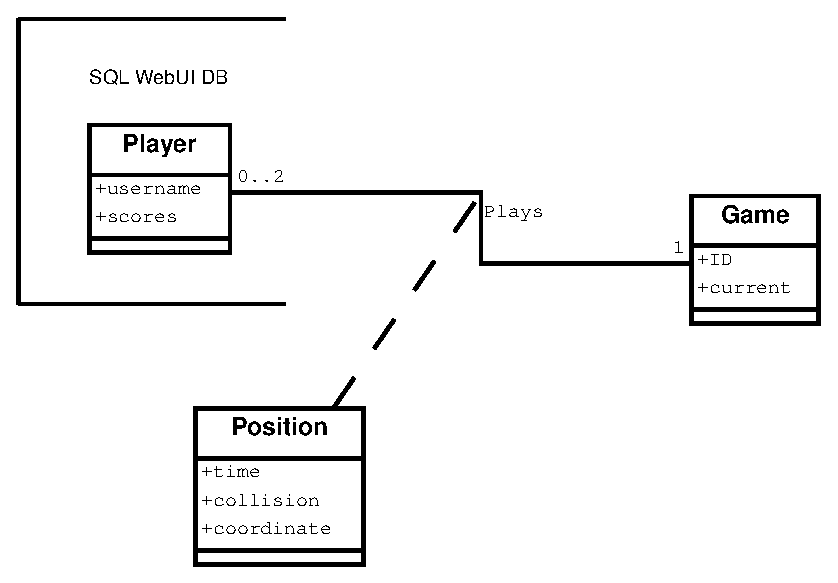
\includegraphics{ERdia.eps} \\


This diagram is loosely modeled off of an E/R diagram. There are two main classes (player and game), and an association complete with a class between them (position). Player is a repository of information that we will communicate with regarding user identity and later update with score information. Our data’s interactions with player class will be minimal but essential for some of the web user interface secondary features, which including information tracking. There can be as little as no players a game up to two, and the position is only important for non-computer players. The game section of the document will hold the gameID and a boolean status of whether or not the game is current, these pieces of information will be added to every game played to ensure better tracking. The boolean ‘current’ will be set from true to false on all documents composing the game when the game ends. The game will also keep track of scores when they are initialized and whenever they are updated.

The position section of the BSON document will experience the most variability, and thus it is attributed as an association class to the plays association. The position is marked most notably by the coordinates of the current player; these coordinates update upon communication with the server. On updating, there will be a time stamp with an imposed index on it. Collision is a String to help during reconstruction that will denote whether or not the movement caused a collision or the ball simply scored, these will be stored as ‘T’ for collision, ‘F’ for no ball interaction, and ‘M’ for if the ball is missed.

The general form of the BSON documents will look something like this:
\begin{verbatim}
var fullDoc = {gameID : Stringnums,
                p1: username, 
                p2: username, 
                p1pos: nums, 
                p2pos: nums, 
                p1score: 0, 
                p2score: 0, 
                collision: String (T/F/M), 
                time: times, 
                current: true
                };
\end{verbatim}
We expect input to look something like this, since we already have the player usernames stored in another document created at the beginning of the game (easily accessible by querying on gameID and searching only for the documents with the ‘p1’ attribute)
\begin{verbatim}
var p1Move =  {gameID: Stringnums,
               p1pos: nums,
               collision: String (T/F/M),
               time: times,
               current: true
               };
\end{verbatim}
On inputting the fact of a player getting a point, we would input a document looking like this. We will merely increment the score by looking back on the latest entry (greatest time stamp) of a player’s score and incrementing it by one
\begin{verbatim}
var p2Miss = {gameID: Stringnums,
              p2:pos,
              collision: M,
              p1score: p1score + 1,
              time: times,
              current: true
              };
\end{verbatim}
The flexibility allowed by BSON documents will allow us to store variable amounts of data at any one given point. MongoDB also has quick information retrieval, allowing us to quickly go back through stored documents upon updating and input.
\subsection{Testing and Verification}

The method used to test our database connection code has primarily consisted of unit testing on the server machine. By using the node-mongodb-native module, any .js files that have calls to the mongodb in them can be run and tested simply by using the ‘node’ command before the file name. Primarily print statements (or, in this case sys.puts(‘ ’); statements) were used to track logical errors. Any compilation on runtime errors were sorted out by referencing the mongodb manuals (as mongojs allows us to write database calls in the mongodb native API) and javascript tutorials. Future integration testing will likely use computer controlled players in games to test data input into the database. After that it will be tested using real player from device inputs.

The method used to test the pong game logic was through the JSBin website. JSBin allows for real time viewing of javascript code and reports errors and warnings in the code as well. From here the server team was able make changes to the code and see how it immediately effected the game logic. JSBin has allowed for learning javascript easier and testing code more efficient.

Server networking was tested primarily with Google Chrome’s JavaScript inspector, as well as the node.js debug mode. There was, of course, plenty of trial-and-error.

\section{Planning and Reflection}
\subsection{Schedule}
\begin{itemize}
	\item Oct 7 -- A database implemented on the server.
	\begin{itemize}
		\item  Be able to have the server do a simple query from the mongoDB database and display it.
		\item This goal was not met on time because the querying protocol was more complex than originally anticipated. It was completed by the following week.
	\end{itemize}
	\item Oct 7 -- Get the server up and running. 
	\begin{itemize}
		\item Be able to have a server that provides text or visual response to simple sample packets from other computers and relays sample information from the database.
		\item This goal was met on time
	\end{itemize}
	\item Oct 11 -- Basic server communication to other devices. 
	\begin{itemize}
		\item Have a proof of concept for devices on the Android and iOS platforms to be able to communicate with the server. Have the clients be able to display information queried from the mongoDB database by communicating with the server.
		\item This goal was not met on time due to unforseen difficulties in handling events. Was met within the week.
	\end{itemize}
	\item Oct 17 -- Simple game engine/logic working.
	\begin{itemize}
		\item Translate the rules of two-player (non-computer opponents) pong into JavaScript code that the server can use. Most likely will test on a browser such as Chrome or Chromium first.
		\item This goal was not met on time because the code we were building out game logic around was difficult to understand, prompting various changes in the source of the programs game logic code.
	\end{itemize}
	\item Nov 4 -- Real-time game streaming on web browsers.
	\begin{itemize}
		\item Be able to watch a game that is happening between two other clients on a third client (most likely a browser at first
		\item Dropped. We no longer believe we have the capacity to impliment streaming. We will instead devote our energies to the replay feature.
	\end{itemize}
	\item Nov 4 -- More robust communication between devices
	\begin{itemize}
		\item Sturdy and smooth communication for devices conversing through the server
	\end{itemize}
	\item Nov 11 -- Be able to replay a game using mongoDB stored information
	\begin{itemize}
		\item Read data stored in the main database and send it to the website interface to be viewed as a replay.
	\end{itemize}
	\item Nov 18 -- Track scores within a game
	\begin{itemize}
		\item During gameplay, incrementation of scores will be sent to the database in order to update the client's interface.
	\end{itemize}
	\item Nov 20 -- Generate a simple computer opponent
	\begin{itemize}
		\item Be able to play against an intelligent AI in 'practice mode.' The AI will do more than simply follow the ball.		
	\end{itemize}
	\item Dec 7 -- Fully functioning back end for Vir-Pong
	\begin{itemize}
		\item Have all functional requirements working optimally and all secondary features integrated in a finished product		
	\end{itemize}
\end{itemize}

\subsection{Challenges}
\begin{itemize}
	\item Communication -- simple communication between the phones and server was incredibly challenging. Getting the communication to register on both the server and the phone took a great deal of debugging. Extra research yielding progress and allowed communication to flow smoothly. In retrospect, it would have probably been beneficial to just pick the most documented and widely-used communication library and worked through it. That being said, the current communication library has been working well since we broke through the "wall" of problems.
	\item Game logic -- the code used as a basis for game logic was not well documented and took a great deal of effort and time to understand the code's implementation, as well as how we could make use of it. It would have probably been better to just write the game logic from scratch, which would not have been too hard since pong was one of the first arcade games ever made.
	
\end{itemize}

\subsection{Future milestones and Member Assignments}
\begin{itemize}
	\item Smooth communication between devices -- one device communicating to another through the server. Daniel will shoulder the primary responsibility and continue to work with the phone groups.
	\item Polished game design -- adding finishing touches to game logic which include scores, timers, and computer opponents. Patrick and Ryan will continue to work on this project. 
	\item Viewing replays -- the web browser interface will be able to view games played previously, as reverse engineered from player position. Shelby will work with the webUI team to continue working on this goal.
\end{itemize}


\section{References}
\subsection{Git and Github}
	\begin{itemize}
		\item Git (http://git-scm.com/) is a distributed version control system that is widely-used in the open source community.
		\item Github (http://github.com/) is a web-based hosting service for projects using git. It provides collaboration tools and many other features such as pull requests and commit management that helps small development groups work efficiently.
		\item The current project repository is hosted on github and collaboration will happen through the web-based UI.
	\end{itemize}
\subsection{node.js}
	\begin{itemize}
		\item node.js (http://nodejs.org/) is an easy-to-learn server-side JavaScript server development environment that supports a myriad of different communication protocols such as HTTP, TCP, and WebSockets.
		\item Will be used as the framework for the server.
		\item express (http://expressjs.com/) is a dead-simple web server application written in node.js.
		\item Socket.io (http://socket.io/) is a cross-platform websocket implementation written in JavaScript for server and client that reverts to Flash and AJAX if WebSockets are not enabled on a certain platform.
	\end{itemize}
\subsection{MongoDB}
	\begin{itemize}
		\item MongoDB (http://mongodb.org/) is a scalable open-source non-relational database with strong node.js support.
		\item mongojs (https://github.com/gett/mongojs) is a wrapper for node-mongodb-native that emulates the mongodb shell API
		\item Node-mongodb-native (https://github.com/christkv/node-mongodb-native/) a node module used to facilitate connection between mongodb and node
		\item Will be used as the main database for storing and retrieving game information.
	\end{itemize}

\subsection{Eclipse}
	\begin{itemize}
		\item Eclipse is an Integrated Development Environment written in Java that provides support for many different programming languages and version control systems through plugins -- A git plugin is available, called Egit (http://eclipse.org/egit/).
		\item Most team members will be using Eclipse IDE for development.
	\end{itemize}
\subsection{Google Docs}
	\begin{itemize}
		\item Google Docs (http://docs.google.com/) is an online document processor with tools similar to Microsoft Word, Powerpoint, and others. It allows for collaboration between different users concurrently on the same document.
		\item Will be used for collaboration on internal documents and documentation.
	\end{itemize}
\subsection{Javascript tutorial}
\begin{itemize}
\item An tutorial (http://www.w3schools.com/js/default.asp) used to learn Javascript and compare against compilation errors.
\end{itemize}

\subsection{Reference Code}

\begin{itemize}
\item The pong file that was modified in order to build the game logic of the pong game (https://github.com/garrettdieckmann/human-pong/blob/master/WebUI/site/http/simppong.html)
\item Bits and pieces of Osmus (https://github.com/borismus/osmus) and NodePong (https://github.com/meetar/NodePong) were used in creating a functional networking framework.
\end{itemize}
\subsection{Javascript Style Guide}
\begin{itemize}
\item A Javascript Style Guide created by Neil Rashbrook (http://neil.rashbrook.org/JS.htm ). We referenced and modified it to create a version applicable to our needs.
\end{itemize}
\end{document}
\subsection{JSBin}
\begin{itemize}
\item JS Bin (http://jsbin.com/odiyej/38/edit) allows for editing and testing of JavaScript and HTML, and includes collaborative functionality. 
\end{itemize}
